% Options for packages loaded elsewhere
\PassOptionsToPackage{unicode}{hyperref}
\PassOptionsToPackage{hyphens}{url}
%
\documentclass[
  english,
  man,man,floatsintext]{apa6}
\usepackage{lmodern}
\usepackage{amssymb,amsmath}
\usepackage{ifxetex,ifluatex}
\ifnum 0\ifxetex 1\fi\ifluatex 1\fi=0 % if pdftex
  \usepackage[T1]{fontenc}
  \usepackage[utf8]{inputenc}
  \usepackage{textcomp} % provide euro and other symbols
\else % if luatex or xetex
  \usepackage{unicode-math}
  \defaultfontfeatures{Scale=MatchLowercase}
  \defaultfontfeatures[\rmfamily]{Ligatures=TeX,Scale=1}
\fi
% Use upquote if available, for straight quotes in verbatim environments
\IfFileExists{upquote.sty}{\usepackage{upquote}}{}
\IfFileExists{microtype.sty}{% use microtype if available
  \usepackage[]{microtype}
  \UseMicrotypeSet[protrusion]{basicmath} % disable protrusion for tt fonts
}{}
\makeatletter
\@ifundefined{KOMAClassName}{% if non-KOMA class
  \IfFileExists{parskip.sty}{%
    \usepackage{parskip}
  }{% else
    \setlength{\parindent}{0pt}
    \setlength{\parskip}{6pt plus 2pt minus 1pt}}
}{% if KOMA class
  \KOMAoptions{parskip=half}}
\makeatother
\usepackage{xcolor}
\IfFileExists{xurl.sty}{\usepackage{xurl}}{} % add URL line breaks if available
\IfFileExists{bookmark.sty}{\usepackage{bookmark}}{\usepackage{hyperref}}
\hypersetup{
  pdftitle={The role of cross-linguistic lexical similarity on bilingual word acquisition},
  pdfauthor={Gonzalo Garcia-Castro1, Daniela Avila-Varela1, \& Nuria Sebastian-Galles1},
  pdflang={en-EN},
  pdfkeywords={lexical acquisition, vocabulary, bilingualism},
  hidelinks,
  pdfcreator={LaTeX via pandoc}}
\urlstyle{same} % disable monospaced font for URLs
\usepackage{graphicx}
\makeatletter
\def\maxwidth{\ifdim\Gin@nat@width>\linewidth\linewidth\else\Gin@nat@width\fi}
\def\maxheight{\ifdim\Gin@nat@height>\textheight\textheight\else\Gin@nat@height\fi}
\makeatother
% Scale images if necessary, so that they will not overflow the page
% margins by default, and it is still possible to overwrite the defaults
% using explicit options in \includegraphics[width, height, ...]{}
\setkeys{Gin}{width=\maxwidth,height=\maxheight,keepaspectratio}
% Set default figure placement to htbp
\makeatletter
\def\fps@figure{htbp}
\makeatother
\setlength{\emergencystretch}{3em} % prevent overfull lines
\providecommand{\tightlist}{%
  \setlength{\itemsep}{0pt}\setlength{\parskip}{0pt}}
\setcounter{secnumdepth}{-\maxdimen} % remove section numbering
% Make \paragraph and \subparagraph free-standing
\ifx\paragraph\undefined\else
  \let\oldparagraph\paragraph
  \renewcommand{\paragraph}[1]{\oldparagraph{#1}\mbox{}}
\fi
\ifx\subparagraph\undefined\else
  \let\oldsubparagraph\subparagraph
  \renewcommand{\subparagraph}[1]{\oldsubparagraph{#1}\mbox{}}
\fi
% Manuscript styling
\usepackage{upgreek}
\captionsetup{font=singlespacing,justification=justified}

% Table formatting
\usepackage{longtable}
\usepackage{lscape}
% \usepackage[counterclockwise]{rotating}   % Landscape page setup for large tables
\usepackage{multirow}		% Table styling
\usepackage{tabularx}		% Control Column width
\usepackage[flushleft]{threeparttable}	% Allows for three part tables with a specified notes section
\usepackage{threeparttablex}            % Lets threeparttable work with longtable

% Create new environments so endfloat can handle them
% \newenvironment{ltable}
%   {\begin{landscape}\begin{center}\begin{threeparttable}}
%   {\end{threeparttable}\end{center}\end{landscape}}
\newenvironment{lltable}{\begin{landscape}\begin{center}\begin{ThreePartTable}}{\end{ThreePartTable}\end{center}\end{landscape}}

% Enables adjusting longtable caption width to table width
% Solution found at http://golatex.de/longtable-mit-caption-so-breit-wie-die-tabelle-t15767.html
\makeatletter
\newcommand\LastLTentrywidth{1em}
\newlength\longtablewidth
\setlength{\longtablewidth}{1in}
\newcommand{\getlongtablewidth}{\begingroup \ifcsname LT@\roman{LT@tables}\endcsname \global\longtablewidth=0pt \renewcommand{\LT@entry}[2]{\global\advance\longtablewidth by ##2\relax\gdef\LastLTentrywidth{##2}}\@nameuse{LT@\roman{LT@tables}} \fi \endgroup}

% \setlength{\parindent}{0.5in}
% \setlength{\parskip}{0pt plus 0pt minus 0pt}

% \usepackage{etoolbox}
\makeatletter
\patchcmd{\HyOrg@maketitle}
  {\section{\normalfont\normalsize\abstractname}}
  {\section*{\normalfont\normalsize\abstractname}}
  {}{\typeout{Failed to patch abstract.}}
\patchcmd{\HyOrg@maketitle}
  {\section{\protect\normalfont{\@title}}}
  {\section*{\protect\normalfont{\@title}}}
  {}{\typeout{Failed to patch title.}}
\makeatother
\shorttitle{Cross-linguistic similarity and  word acquisition}
\keywords{lexical acquisition, vocabulary, bilingualism\newline\indent Word count: X}
\usepackage{lineno}

\linenumbers
\usepackage{csquotes}
\ifxetex
  % Load polyglossia as late as possible: uses bidi with RTL langages (e.g. Hebrew, Arabic)
  \usepackage{polyglossia}
  \setmainlanguage[]{english}
\else
  \usepackage[shorthands=off,main=english]{babel}
\fi
\newlength{\cslhangindent}
\setlength{\cslhangindent}{1.5em}
\newenvironment{cslreferences}%
  {\setlength{\parindent}{0pt}%
  \everypar{\setlength{\hangindent}{\cslhangindent}}\ignorespaces}%
  {\par}

\title{The role of cross-linguistic lexical similarity on bilingual word acquisition}
\author{Gonzalo Garcia-Castro\textsuperscript{1}, Daniela Avila-Varela\textsuperscript{1}, \& Nuria Sebastian-Galles\textsuperscript{1}}
\date{}


\authornote{

Campus de Ciutadella, Universitat Pompeu Fabra, 08005, Barcelona, Spain

Correspondence concerning this article should be addressed to Gonzalo Garcia-Castro, Ramon Trias Fargas, 25-27, 08005 Barcelona, Spain. E-mail: \href{mailto:gonzalo.garciadecastro@upf.edu}{\nolinkurl{gonzalo.garciadecastro@upf.edu}}

}

\affiliation{\vspace{0.5cm}\textsuperscript{1} Center for Brain and Cognition, Universitat Pompeu Fabra, Barcelona, Spain}

\abstract{
Bilinguals face the challenging task of learning words from languages with overlapping phonologies. Floccia et al.~(2018) reported larger vocabulary sizes for 24-month-old bilinguals that were learning languages that shared a greater amount of cognates (e.g., English-Dutch). The mechanisms underlying this effect remain unknown. We explore two compatible scenarios. First, we test whether cognates are learnt earlier than non-cognates. This would account for the difference in vocabulary size associated to the amount of shared cognates across languages. Second, we explore the possibility that the word-forms of one language interact with those form the other language, scaffolding the acquisition of their translation equivalents when their phonologies overlap. This mechanism, in line with the parallel activation account of bilingual speech perception, would provide a plausible explanation to why cognates are acquired ealier by bilinguals. We developed an online tool to collect parental reports of receptive and productive vocabularies from children learning Catalan and/or Spanish, and present data on receptive and productive vocabulary of bilingual toddlers aged 12 to 34 months.
}



\begin{document}
\maketitle

\hypertarget{introduction}{%
\section{Introduction}\label{introduction}}

Learning words involves two key steps: (1) the encoding of a word form (e.g, /dɒɡ/)
and (2) its association with a referent (e.g., a DOG). There is evidence that word learning occurs at early ages: six-month-old infants show a preference toward named pictures, relative to unnamed pictures displayed side-by-side ({\textbf{???}}). At 7.5 months, the phonological representations of familiar words seem to be quite detailed, as infants show evidence of recognition when the whole word is uttered ({\textbf{???}}), as opposed to when only part of the word is uttered. At 12 months, infants show sensitivity to both vowel and consonant mispronunciations ({\textbf{???}}), looking shorter to named pictures when their label is mispronounced. Remarkable as it is, the phonological specificity of infants' lexical entries is only the foundation of following developmental milestones. One of them, central to this study, is the emergence of excitatory and inhibitory links between word representations, which represents one of the essential characteristics of the adult lexicon ({\textbf{???}}).

Words are not learnt in isolation, but in contexts rich in word tokens and referents. The structure of toddlers' lexicon reflects this high connectivity ({\textbf{???}}; {\textbf{???}}; {\textbf{???}}). At 18 months, infants' recognition of spoken words is sensitive to phonological priming effects, suggesting that their lexical entries are phonological linked, and co-activated during speech processing ({\textbf{???}}; {\textbf{???}}). The emergence of semantic links in the developing lexicon occurs somewhat later, at 24 months of age, when infants show sensitivity to semantic priming ({\textbf{???}}; {\textbf{???}}; {\textbf{???}}), and show evidence of inhibitory links between lexical-semantic entries ({\textbf{???}}). By 24 months, toddlers' recognition of familiar words also seems to follow a hierarchical fashion, as revealed by their sensitivity to the phonology and semantic similarity of distractor pictures presented along the named picture: the interference of phonological distractors is stronger at earlier stages of spoken word recognition, that of semantic distractors is stronger at later stages ({\textbf{???}}). Vocabulary size predicts the emergence and the strength of these effects: 18 months-old toddlers are sensitive to semantic priming and interference too, provided they know a similar amount of words ({\textbf{???}}; {\textbf{???}}), and the strength of the phonological and semantic distractors during spoken word recognition grows stronger along the vocabulary size of the toddlers. This suggests that the emergence of rich lexical networks -- both at the phonological and the semantic levels -- grows as a function of the number of words acquired by the toddler.

The structure of the lexicon also impacts the order of acquisition of new words. Words that share a high degree of phonological and/or semantic overlap with words already acquired are more likely to be acquired next (Hills, Maouene, Maouene, Sheya, \& Smith, 2009). ({\textbf{???}}) and ({\textbf{???}}) showed that the connectivity of a given semantic category (i.e., animals) in a child's lexicon predicts a better performance in a disambiguation task, where participants are presented with a novel label in the presence of a familiar and a novel object: infants show stronger looking preference for the novel object if it belonged to a category for which many words had already been acquired. This points to the structure of the lexicon facilitating the strategies children engage during word learning.

The case of bilingual children (here defined as those learning two languages from birth) presents an opportunity to study how lexical acquisition takes placed under a more complex environment, as they face the challenge of learning two distinct sets of words -- one for each language -- that partially overlap in sound and meaning.

EARLY STAGES IN BILINGUAL LANGUAGE ACQUISITION

When compared to their monolingual peers, they know fewer words only when just on language is considered (e.g., English monolinguals know more words in English than English-Spanish bilinguals). When both languages are taken into account, bilingual children seem to know, at least, as many words as monolinguals do ({\textbf{???}}; {\textbf{???}}; Ben-Zeev, 1977; Bialystok, Luk, Peets, \& Yang, 2010; Blom et al., 2019; Core, Hoff, Rumiche, \& Señor, 2013; Fernandez, Pearson, Umbel, Oiler, \& Molinet-Molina, 1992; Hoff et al., 2012; Hoff, Rumiche, Burridge, Ribot, \& Welsh, 2014; Pearson \& Fernández, 1994; but see Pearson, Fernández, \& Oller, 1993; Houwer, Bornstein, \& Putnick, 2014).

Floccia et al. (2018), gathered parental vocabulary estimates (Hamilton, Plunkett, \& Schafer, 2000) from a large sample of 24-month-old toddlers learning English and an additional language (from a pool of 13 linguistically diverse languages). They computed the average phonological similarity between translation equivalents (TEs from now on; e.g., \emph{table} in English and \emph{tafel} in Dutch) for each pair of languages, and found a positive association between this measure of phonological similarity and participants' productive vocabulary sizes in their additional language. Using a similar measure of lexical similarity, Blom et al. (2019) extended these results to bilingual children aged three to 10, and reported a positive association between the lexical distance and comprehensive vocabulary size: bilinguals learning lexically close languages showed similar vocabulary sizes to those of monolinguals, but those learning the more distant languages showed lower vocabulary sizes.

These results suggest that linguistic distance between languages plays an important role during bilingual lexical acquisition, and that this effect operates within TEs. What mechanisms underlie this effect, and why they seem to operate differently across comprehension and production, or across the dominant and the non-dominant language, remain open issues. Floccia et al. (2018) pointed to parallel activation as a candidate mechanism behind this facilitation effect. The parallel activation principle suggests that bilinguals activate lexical representations in a language non-selective way: during the comprehension or production of a word in one language (e.g., \emph{cat}, in English) its corresponding translation in the other language is activated too {[}e.g., \emph{gato}, in Spanish. There is a vast body of evidence supporting language non-selective lexical access in both adults (e.g., Dell \& O'Seaghdha, 1991; {\textbf{???}}; Bobb, Von Holzen, Mayor, Mani, \& Carreiras, 2020; Costa \& Caramazza, 2000; Dijkstra, 2005; Hoshino \& Kroll, 2008; Kroll, Gullifer, \& Rossi, 2013; Singh, 2014; Thierry \& Wu, 2007; Von Holzen, Fennell, \& Mani, 2019; Yudes, Macizo, \& Bajo, 2010; see Costa, Santesteban, \& Caño, 2005 for review), and children (e.g.~Von Holzen \& Mani, 2012; {\textbf{???}}; {\textbf{???}}; {\textbf{???}}). A critical implication of parallel activation is that the word form (i.e., phonology, orthography, etc.) of both translation equivalents are available to each other, impacting the comprehension or production dynamic of any of them.

Floccia et al. (2018) argue that the degree of phonological similarity between TEs (\emph{cognateness} from now on) of both languages should lead to increased parallel activation of both languages during language exposure, facilitating the acquisition of words in both languages, and leading participants leading two lexically close languages to show larger vocabulary sizes than those learning two lexically distant languages. This account, however, neglects the fact that for parallel activation to take place and play a facilitation role, lexical representations of both pairs of the TE must have been already established in the lexicon, and their corresponding phonological forms must have been encoded. This is not the case during lexical acquisition, where at least one of the members of the pair has not being acquired yet. A more lenient definition of parallel activation could adjust to the context of lexical acquisition more easily: when only one of the members of the TE has been acquired, its lexical representation is activated when, in the presence of its referent, a phonologically similar label is uttered. Consider the case of a Catalan-Spanish bilingual that has already learned the word \emph{gat} (Catalan for \emph{cat}), but not \emph{gato} (in Spanish). It is possible that, when presented with \emph{gato} in the presence of a cat, she maps this novel label to the familiar word \emph{gat}, and creates a lexical representation for \emph{gato} as a synonym for \emph{gat}. The case of a non-cognate is differing. Consider now the case of a toddler that has already learnt \emph{gos} (Catalan for \emph{dog}), but not \emph{perro} (Spanish). In this case, it would not be possible to map both labels via phonology, give their lack of phonological similarity.

Under this account, cognates (i.e., phonologically similar TEs) would be acquired earlier than non-cognates, but this effect would only play a role once one of the members of the TE has been acquired. The evidence supporting an earlier age of acquisition of cognates relative to non-cognates if sparse. Schelletter (2002) reported a longitudinal case-study of a German/English child who produced cognate TEs earlier than non-cognate TE. Bosch and Ramon-Casas (2014), showed converging results from a sample of 48 monolingual and bilingual infants aged 24 months. The low number of words included in the analyses of both studies, and the lack of adjustment for lexical frequency, limits severely the strength of any conclusions concerning the difference in age of acquisition of cognates and non-cognates. On the other hand Floccia et al. (2018) worked with aggregated estimates of participants' vocabulary size, losing item-level information that could provide information about change in age of acquisition of TEs associated with their degree of phonological similarity. Therefore, their results can only be considered as compatible with cognateness playing a role on age of acquisition. In this study, we aimed at overcoming these pitfalls by using unaggregated data from individual responses, testing the role of cognateness explicitly and adjusting for lexical frequency.

It also follows from the fact that cognateness operates \emph{within} TEs that the effect of cognateness can only play a role once one of the members of the TE has been acquired, and its phonological form is available during the acquisition of its translation. Words that belong to the language of most exposure (dominant language) are likely to be acquired earlier than words in the non-dominant language (Floccia et al., 2018). ({\textbf{???}}) tested Dutch-Frisian bilingual children aged 2.5 to four years in a comprehension task (PPVT-NL) that involved Frisian words with different degrees of phonological similarity with their Dutch TE. Infants with lower exposure to Frisian showed a better performance for words with high similarity, while no such benefit was found in children who were exposed mostly to Frisian. This suggests that infants that were mostly exposed to Dutch used the phonology of dutch words when processing Frisian words, as revealed by a better performance for cognates than for non-cognates.
A study by ({\textbf{???}}) showed that the degree of phonological similarity between
the performance of was better for cognates than for non-cognates, only for those children

Finally, previous studies have reported that the properties that describe the form of a word play a stronger role in production than comprehension than in production. This is the case of the number of phonemes (Braginsky, Yurovsky, Marchman, \& Frank, 2019), phonological neighbourhood density (Jones \& Brandt, 2019). These results converge with Floccia et al. (2018)'s finding that the effect of the average cognateness between languages was larger in production than in comprehension\footnote{Although Bosch and Ramon-Casas (2014) found that participants in their sample produced cognates earlier than non-cognates, no analyses were conducted on comprehensive data, and therefore they cannot be taken as supporting evidence for a larger effect of cognateness on production than in comprehension}. Accordingly, we expected the role of cognateness to be more central in production than in comprehension.

In summary, we investigated the effect of cognateness on the probability of acquisition of TEs, and predicted that (1) cognate TEs are acquired earlier than non-cognate TEs, that this effect will be larger in the dominant than in the non-dominant language, and larger in production than in comprehension.

\hypertarget{method}{%
\section{Method}\label{method}}

\hypertarget{participants}{%
\subsection{Participants}\label{participants}}

We collected data from 349 bilinguals (167 female), from the Metropolitan Area of Barcelona, between 28th October, 2019 and 09th January, 2021. All families gave informed consent before participating. This study was approved by the Comitè d'Ètica de la Investigació amb Medicaments (CEIm) from Hospital del Mar (Barcelona, Spain), code XXXXXXXXX. We assessed toddlers' language profile asking parents for an estimated proportion of exposure to each language. We excluded participants with \textgreater10\% exposure to a third language. Fig. \ref{tab:lps} illustrates the distribution of participants across language profiles and ages.

\hypertarget{questionnaire}{%
\subsection{Questionnaire}\label{questionnaire}}

We implemented an on-line questionnaire using \texttt{formr} (Arslan, Walther, \& Tata, 2020), divided in three forms: a (1) language questionnaire, a (2) demographic survey, and a (3) Catalan and a Spanish vocabulary checklists. Vocabulary checklists followed a similar structure as the Oxford Communicative Developmental Inventory (Hamilton et al., 2000) and consisted in two lists of words, one in Catalan and one in Spanish). Items in one language were translation equivalents of the items in the other (e.g., whenever \emph{gos} {[}dog{]} was included in the Catalan inventory, the word \emph{perro} was included in the Spanish inventory), roughly following a one-to-one mapping. When there were two acceptable translation equivalents for a given word, we included both (e.g., Catalan \emph{acabar} {[}\emph{to finish}{]} and Spanish \emph{acabar} and \emph{terminar}), or merged them into the same one (e.g., Spanish \emph{mono} {[}\emph{monkey}{]} and Catalan \emph{mono/mico}). We included items from a diverse sample of 26 semantic/functional categories (see Appendix 1). We discarded the following categories: adverbs, auxiliary words, connectives, interjections and games and routines. The Catalan inventory contained 778 items (196 cognates, 582 non-cognates) and the Spanish inventory contained 781 (197 cognates, 584 non-cognates).

For each word in the vocabulary checklists, we asked parents to report whether their child was able to understand it, understand and say it, or did not understand or say it (marked by default). Participants filled a long or a short version of the questionnaire. Participants presented with the long version filled a list of 800 translation equivalents (800 items in Catalan and 800 items in Spanish), while participants presented with a short were randomly allocated into one of four list of items. Each list contained a different set of \textasciitilde400 translation equivalents (\textasciitilde400 in Catalan, \textasciitilde400 in Spanish). Semantic/functional categories with less than 16 items--thus resulting in less than four items after dividing it in four lists - were not divided in the short version of the questionnaire: all of their items were included in the four lists. Another subset of items that were part of the trial lists of some experiments in the lab were also included in all versions. Table 2 in Appendix 1 shows the distribution of items across questionnaire versions. We excluded from the analysis multi-word items (e.g., \emph{barrita de cereales} {[}cereal bar{]}) and items that included more than one word-form (e.g., \emph{mono / mico}). Table \ref{tab:itemsinfo} shows the classification of items in cognates and non-cognates and their frequency scores across the four lists of the inventories.

\hypertarget{data-analysis}{%
\subsection{Data analysis}\label{data-analysis}}

We gathered 181587 responses. Translation equivalents received an average of 386.36 (\emph{SD} = 228.76, , Max = 698), both languages summed together. We modelled the probability of responses (\(y_i\)) belonging to any of the three possible categories \(k\)--1 = \emph{No} or say, 2 = \emph{Understands}, and 3 = \emph{Understands and Says}-- using an ordinal regression model with a cumulative logit link function (Agresti, 2010; Bürkner \& Vuorre, 2019). This model estimates the probability of response \(y_i\) to belong to category \(k\) or lower. In our case, this will result in the estimation of the probability of \(y_i \leq 1\), \(y_i \leq 2\), and \(y_i \leq 3\), where

\[
p_k = Pr(y_i = k) = Pr(y_i \leq k) - Pr(y_i \leq k-1).
\]

We include several predictors of interest to adjust this probability to participants' and items' (lexical frequency, dominance, cognateness) characteristics. These predictors are:

\begin{itemize}
\tightlist
\item
  Age of participant in months (\texttt{age}, \(Age\)) calculated as the difference in days between participants' birth date and questionnaire completion divided by 30 and centred around the mean
\item
  Degree of bilingualism of participant (\texttt{bilingualism}, \(Bilingualism\)) computed as the percentage of exposure to a second language (Spanish for participants exposed to \textgreater50\% to Catalan an \emph{vice versa}) rounded to units and centered around the mean
\item
  Lexical frequency of item (\texttt{frequency}, \(Frequency\)) retrieved from SUBTLEX-CAT (Boada, Guasch, Haro, Demestre, \& Ferré, 2019) for Catalan words and from SUBTLEX-ESP (Cuetos, Glez-Nosti, Barbón, \& Brysbaert, 2011) for Spanish words, expressed as Zipf scores (Heuven, Mandera, Keuleers, \& Brysbaert, 2014), and centred around the mean
\item
  Language the item belongs to (\texttt{dominance}, \(Dominance\)) labelled as \texttt{L1} if the item belongs to the dominant language (e.g., a Catalan item is labelled as \texttt{L1} for Catalan-dominant participants and as \texttt{L2} for Spanish-dominant participants), coded as \texttt{L2} = -0.5 and \texttt{L1} = 0.5
\item
  Cognateness of the item (\texttt{cognate}, \(Cognate\)), coded as \texttt{Non-cognate} = -0.5 and \texttt{Cognate} = 0.5
\end{itemize}

We adopted a Bayesian approach toward statistical inference, which allows to (1) incorporate previous domain knowledge into the inference process implementing the Bayes theorem, and (2) to quantify the uncertainty associated to the estimated parameters in our model. Our extended model can be formalised as follows:

\[
\begin{aligned}
y_i \sim Ordered(p) \\
log\frac{Pr(y_i \leq k)}{1-Pr(y_i \leq k)} &= \alpha_k - \dots \\
& \beta_1 \times Age_i + \dots \\
& \beta_2 \times Frequency_i + \dots \\
& \beta_3 \times Dominance_i + \dots \\
& \beta_4 \times Bilingualism_i + \dots \\
& \beta_5 \times Cognate_i + \dots \\
& \beta_6 \times (Dominance_i \times Bilingualism_i) + \dots \\
& \beta_7 \times (Dominance_i \times Cognate_i) + \dots \\
& \beta_8 \times (Bilingualism_i \times Cognate_i) + \dots \\
& \beta_9 \times (Dominance_i \times Bilingualism_i \times Cognate_i), \\
\alpha \sim Normal(0, 10) \\
\beta_{0-9} \sim Normal(0, 10)
\end{aligned}
\]

Where:

\begin{itemize}
\tightlist
\item
  \(k\) is one of the possible categories (coded as ) responses can take
\item
  \(y_i\) is the \texttt{response} value of observation \(i\)
\item
  \(\alpha_k\) is the mean probability of responses to belong to category \(k\)
\item
  \(\beta_{1, \dots, 9}\) are the coefficients of the predictors
\end{itemize}

We implemented the model using the R package \texttt{brms} (Bürkner, 2017) as \texttt{response\ \textasciitilde{}\ \ age\ +\ frequency\ +\ dominance*bilingualism*cognate}, running four MCMC sampling chains with 4,000 iterations (including 2,000 warm-up iterations per chain). We used weakly regularising prior for the parameters in our model, given that its weight in the estimation of the posterior will be marginal due to the large amount of observations introduced in the model. We report the 95\% credible intervals (CrI) of the estimated posterior distribution of each parameter, which denotes a range of values we are 95\% certain contain the true value, given our prior and observed data. We report analyses on the probability scale, having transformed the log-odds returned by the model using an inverse logit transformation.

We fit increasingly simpler models dropping predictors one by one in the following order: (1) \texttt{dominance:bilingualism:cognate}, (2) \texttt{bilingualism:cognate}, (3) \texttt{dominance:cognate:}, (4) \texttt{cognate}, (5) \texttt{dominance:bilingualism}, (6) \texttt{bilingualism}, (7) \texttt{dominance}, (8) \texttt{frequency}, and (9) \texttt{age}. We compared all models using leave-one-out cross-validation (LOO-CV) (Vehtari, Gelman, \& Gabry, 2017)\footnote{Due to the high computational cost associated with a large dataset, we used a sub-sampling approach for performing Bayesian LOO with 1000 samples (Magnusson, Andersen, Jonasson, \& Vehtari, 2019)}. We then explored the posterior distribution of each parameter in the model that fitted the data the best, computing the 95\% credible intervals and testing whether this interval excluded 0. We performed follow-up tests on interactions whose 95\% credible interval excluded 0 by comparing the 95\% credible interval of their estimated marginal means using the \texttt{emmeans} package (Lenth, 2020). Data processing and visualisation was done in R (R Core Team, 2020) using the \texttt{tidyverse} family of packages (Wickham et al., 2019), and posterior samples were extracted using the \texttt{tidybayes} R package (Kay, 2020).

\hypertarget{results}{%
\section{Results}\label{results}}

Table 2 summarises shows the outcome of the LOO-CV model comparison. The extended model was most favoured by the data.

\captionsetup[table]{labelformat=empty,skip=1pt}
\begin{longtable}{crrrrr}
\toprule
& & & & \multicolumn{2}{c}{\textbf{Comparison}} \\ 
 \cmidrule(lr){5-6}
\textbf{Model} & \textbf{ELPD}\textsuperscript{a} & \textbf{SE}\textsuperscript{b} & \textbf{p}\textsuperscript{c} & \emph{LOOdiff} & \emph{SEdiff} \\ 
\midrule
\textasciitilde  1 (intercept only) & $-157,272.37$ & $250.56$ & $12.00$ & $0.00$ & 0.0000 \\ 
... + age & $-157,308.76$ & $250.47$ & $10.37$ & $36.39$ & 354.2836 \\ 
... + frequency & $-157,318.93$ & $250.45$ & $9.93$ & $46.56$ & 354.2703 \\ 
... + dominance & $-157,463.31$ & $250.25$ & $8.08$ & $190.94$ & 354.1293 \\ 
... + bilingualism & $-157,472.54$ & $250.29$ & $7.67$ & $200.17$ & 354.1564 \\ 
... + dominance:bilingualism & $-158,724.35$ & $246.22$ & $6.33$ & $1,451.98$ & 351.2863 \\ 
... + cognate & $-159,063.42$ & $245.10$ & $5.09$ & $1,791.06$ & 350.5085 \\ 
... + dominance:cognate & $-161,704.16$ & $237.62$ & $3.95$ & $4,431.79$ & 345.3184 \\ 
... + bilingualism:cognate & $-165,570.87$ & $228.08$ & $3.13$ & $8,298.50$ & 338.8223 \\ 
... + dominance:bilingualism:cognate & $-184,511.91$ & $172.86$ & $2.04$ & $27,239.54$ & 304.4033 \\ 
\bottomrule
\end{longtable}
\vspace{-5mm}
\begin{minipage}{\linewidth}
\textsuperscript{a}ELPD: theoretical expected log pointwise predictive density for a new dataset, as estimated using Bayesian LOO-CV \\ 
\textsuperscript{b}SE: standard error of the ELPD \\ 
\textsuperscript{c}p: effective number of parameters \\ 
\end{minipage}

Table 3 shows the mean and 95\% CrI of each regression coefficient of the best fitting model.

\captionsetup[table]{labelformat=empty,skip=1pt}
\begin{longtable}{lrrrrrr}
\toprule
& \multicolumn{3}{c}{\textbf{Odds Ratio}} & \multicolumn{3}{c}{\textbf{Probability}} \\ 
 \cmidrule(lr){2-4}\cmidrule(lr){5-7}
\textbf{Coefficient} & \emph{Mean} & \emph{SE}\textsuperscript{1} & \emph{95\% CrI}\textsuperscript{2} & \emph{Mean} & \emph{SE} & \emph{95\% CrI} \\ 
\midrule
Intercept 1 (Understands) & $1.12$ & $1.01$ & $1.11$–$1.14$ & $0.53$ & $0.50$ & $0.53$–$0.53$ \\ 
Intercept 2 (Understands \& Says) & $5.31$ & $1.01$ & $5.24$–$5.38$ & $0.84$ & $0.50$ & $0.84$–$0.84$ \\ 
Age & $1.16$ & $1.00$ & $1.16$–$1.17$ & $0.54$ & $0.50$ & $0.54$–$0.54$ \\ 
Frequency & $1.86$ & $1.01$ & $1.83$–$1.88$ & $0.65$ & $0.50$ & $0.65$–$0.65$ \\ 
Dominance & $2.27$ & $1.01$ & $2.22$–$2.32$ & $0.69$ & $0.50$ & $0.69$–$0.70$ \\ 
Bilingualism & $1.10$ & $1.00$ & $1.09$–$1.11$ & $0.52$ & $0.50$ & $0.52$–$0.53$ \\ 
Cognate & $1.08$ & $1.01$ & $1.06$–$1.10$ & $0.52$ & $0.50$ & $0.51$–$0.52$ \\ 
Dominance * Bilingualism & $0.73$ & $1.01$ & $0.73$–$0.74$ & $0.42$ & $0.50$ & $0.42$–$0.43$ \\ 
Dominance * Cognate & $0.68$ & $1.02$ & $0.65$–$0.71$ & $0.40$ & $0.51$ & $0.39$–$0.42$ \\ 
Bilingualism * Cognate & $0.97$ & $1.01$ & $0.96$–$0.98$ & $0.49$ & $0.50$ & $0.49$–$0.50$ \\ 
Dominance * Bilingualism * Cognate & $1.13$ & $1.01$ & $1.10$–$1.15$ & $0.53$ & $0.50$ & $0.52$–$0.54$ \\ 
\bottomrule
\end{longtable}
\vspace{-5mm}
\begin{minipage}{\linewidth}
\textsuperscript{1}SE: Standard Error of the mean \\ 
\textsuperscript{2}95\% CrI: 95\% credible interval \\ 
\end{minipage}

\begin{figure}

{\centering 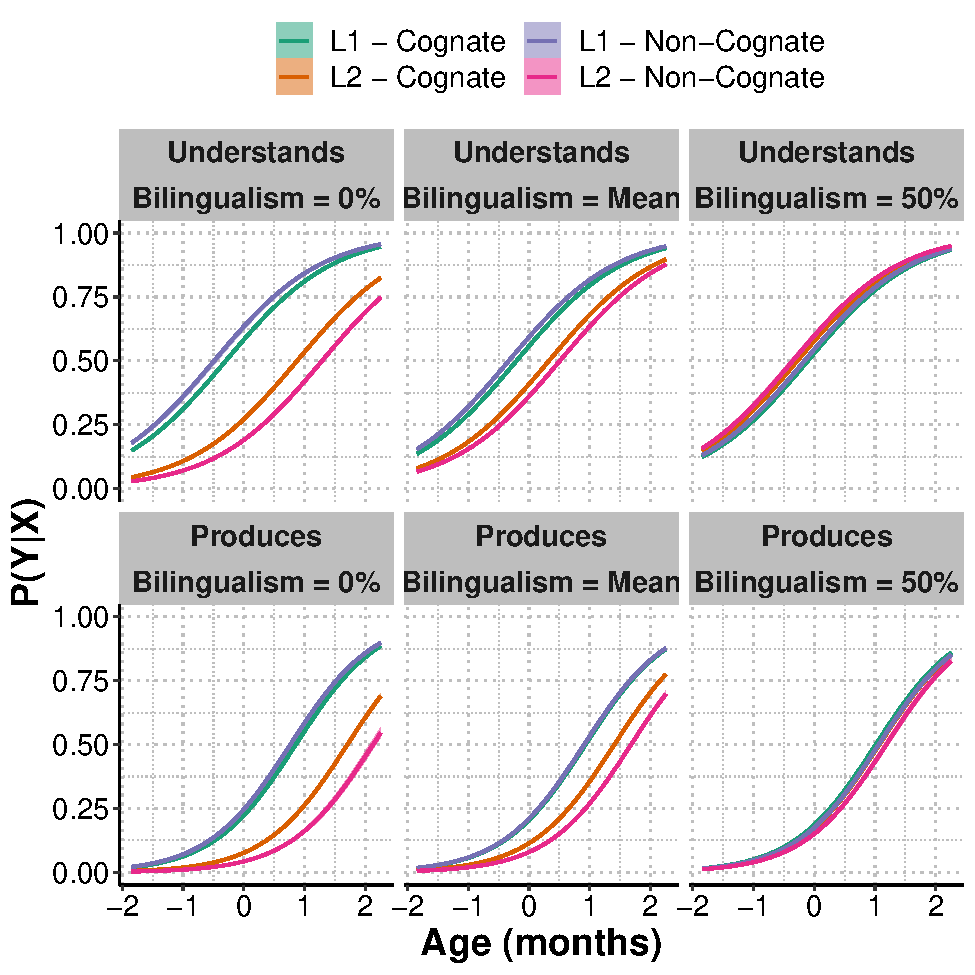
\includegraphics[width=20cm]{trajectories_manuscript_files/figure-latex/marginalmeans-1} 

}

\caption{Mean posterior probability and 95\% CrI of responses, conditional to Dominance, Bilingualism, and Cognate.}\label{fig:marginalmeans}
\end{figure}

\hypertarget{discussion}{%
\section{Discussion}\label{discussion}}

\hypertarget{references}{%
\section{References}\label{references}}

\begingroup
\setlength{\parindent}{-0.5in}
\setlength{\leftskip}{0.5in}

\hypertarget{refs}{}
\begin{cslreferences}
\leavevmode\hypertarget{ref-agresti_analysis_2010}{}%
Agresti, A. (2010). \emph{Analysis of ordinal categorical data} (Vol. 656). John Wiley \& Sons.

\leavevmode\hypertarget{ref-arslan_formr_2020}{}%
Arslan, R. C., Walther, M. P., \& Tata, C. S. (2020). Formr: A study framework allowing for automated feedback generation and complex longitudinal experience-sampling studies using R. \emph{Behavior Research Methods}, \emph{52}(1), 376--387. \url{https://doi.org/10.3758/s13428-019-01236-y}

\leavevmode\hypertarget{ref-ben-zeev_influence_1977}{}%
Ben-Zeev, S. (1977). The Influence of Bilingualism on Cognitive Strategy and Cognitive Development. \emph{Child Development}, \emph{48}(3), 1009--1018. \url{https://doi.org/10.2307/1128353}

\leavevmode\hypertarget{ref-bialystok_receptive_2010}{}%
Bialystok, E., Luk, G., Peets, K. F., \& Yang, S. (2010). Receptive vocabulary differences in monolingual and bilingual children. \emph{Bilingualism: Language and Cognition}, \emph{13}(4), 525--531. \url{https://doi.org/10.1017/S1366728909990423}

\leavevmode\hypertarget{ref-blom_cross-language_2019}{}%
Blom, E., Boerma, T., Bosma, E., Cornips, L., Heuij, K. van den, \& Timmermeister, M. (2019). Cross-language distance influences receptive vocabulary outcomes of bilingual children. \emph{First Language}, 0142723719892794. \url{https://doi.org/10.1177/0142723719892794}

\leavevmode\hypertarget{ref-boada_subtlex-cat_2019}{}%
Boada, R., Guasch, M., Haro, J., Demestre, J., \& Ferré, P. (2019). SUBTLEX-CAT: Subtitle word frequencies and contextual diversity for Catalan. \emph{Behavior Research Methods}. \url{https://doi.org/10.3758/s13428-019-01233-1}

\leavevmode\hypertarget{ref-bobb_co-activation_2020}{}%
Bobb, S. C., Von Holzen, K., Mayor, J., Mani, N., \& Carreiras, M. (2020). Co-activation of the L2 during L1 auditory processing: An ERP cross-modal priming study. \emph{Brain and Language}, \emph{203}, 104739. \url{https://doi.org/10.1016/j.bandl.2019.104739}

\leavevmode\hypertarget{ref-bosch_first_2014}{}%
Bosch, L., \& Ramon-Casas, M. (2014). First translation equivalents in bilingual toddlers' expressive vocabulary: Does form similarity matter? \emph{International Journal of Behavioral Development}, \emph{38}(4), 317--322. \url{https://doi.org/10.1177/0165025414532559}

\leavevmode\hypertarget{ref-braginsky_consistency_2019}{}%
Braginsky, M., Yurovsky, D., Marchman, V. A., \& Frank, M. C. (2019). Consistency and Variability in Children's Word Learning Across Languages. \emph{Open Mind}, \emph{3}, 52--67. \url{https://doi.org/10.1162/opmi_a_00026}

\leavevmode\hypertarget{ref-burkner_brms_2017}{}%
Bürkner, P.-C. (2017). Brms: An R Package for Bayesian Multilevel Models Using Stan. \emph{Journal of Statistical Software}, \emph{80}(1), 1--28. \url{https://doi.org/10.18637/jss.v080.i01}

\leavevmode\hypertarget{ref-burkner_ordinal_2019}{}%
Bürkner, P.-C., \& Vuorre, M. (2019). Ordinal regression models in psychology: A tutorial. \emph{Advances in Methods and Practices in Psychological Science}, \emph{2}(1), 77--101.

\leavevmode\hypertarget{ref-core_total_2013}{}%
Core, C., Hoff, E., Rumiche, R., \& Señor, M. (2013). Total and Conceptual Vocabulary in Spanish--English Bilinguals From 22 to 30 Months: Implications for Assessment. \emph{Journal of Speech, Language, and Hearing Research}, \emph{56}(5), 1637--1649. \url{https://doi.org/10.1044/1092-4388(2013/11-0044)}

\leavevmode\hypertarget{ref-costa_lexical_2000}{}%
Costa, A., \& Caramazza, A. (2000). Lexical access in speech production: The bilingual case. \emph{Psicológica}, \emph{21}(2), 403--437.

\leavevmode\hypertarget{ref-costa_facilitatory_2005}{}%
Costa, A., Santesteban, M., \& Caño, A. (2005). On the facilitatory effects of cognate words in bilingual speech production. \emph{Brain and Language}, \emph{94}(1), 94--103.

\leavevmode\hypertarget{ref-cuetos_subtlex-esp_2011}{}%
Cuetos, F., Glez-Nosti, M., Barbón, A., \& Brysbaert, M. (2011). SUBTLEX-ESP: Spanish word frequencies based on film subtitles. \emph{Psicológica}, \emph{32}(2), 133--143.

\leavevmode\hypertarget{ref-dell_mediated_1991}{}%
Dell, G. S., \& O'Seaghdha, P. G. (1991). Mediated and convergent lexical priming in language production: A comment on levelt et al (1991).

\leavevmode\hypertarget{ref-dijkstra_bilingual_2005}{}%
Dijkstra, T. (2005). Bilingual Visual Word Recognition and Lexical Access. In \emph{Handbook of bilingualism: Psycholinguistic approaches} (pp. 179--201). New York, NY, US: Oxford University Press.

\leavevmode\hypertarget{ref-fernandez_bilingual_1992}{}%
Fernandez, M. C., Pearson, B. Z., Umbel, V. M., Oiler, D. K., \& Molinet-Molina, M. (1992). Bilingual Receptive Vocabulary in Hispanic Preschool Children. \emph{Hispanic Journal of Behavioral Sciences}, \emph{14}(2), 268--276. \url{https://doi.org/10.1177/07399863920142006}

\leavevmode\hypertarget{ref-floccia_i_2018}{}%
Floccia, C., Sambrook, T. D., Luche, C. D., Kwok, R., Goslin, J., White, L., \ldots{} Plunkett, K. (2018). I: Introduction. \emph{Monographs of the Society for Research in Child Development}, \emph{83}(1), 7--29. \url{https://doi.org/10.1111/mono.12348}

\leavevmode\hypertarget{ref-hamilton_infant_2000}{}%
Hamilton, A., Plunkett, K., \& Schafer, G. (2000). Infant vocabulary development assessed with a british communicative development inventory. \emph{Journal of Child Language}, \emph{27}(3), 689--705.

\leavevmode\hypertarget{ref-heuven_subtlex-uk_2014}{}%
Heuven, W. J. B. van, Mandera, P., Keuleers, E., \& Brysbaert, M. (2014). Subtlex-UK: A New and Improved Word Frequency Database for British English: \emph{Quarterly Journal of Experimental Psychology}. Retrieved from \url{https://journals.sagepub.com/doi/10.1080/17470218.2013.850521}

\leavevmode\hypertarget{ref-hills_longitudinal_2009}{}%
Hills, T. T., Maouene, M., Maouene, J., Sheya, A., \& Smith, L. (2009). Longitudinal Analysis of Early Semantic Networks Preferential Attachment or Preferential Acquisition? \emph{Psychological Science}, \emph{20}(6), 729--739. \url{https://doi.org/10.1111/j.1467-9280.2009.02365.x}

\leavevmode\hypertarget{ref-hoff_dual_2012}{}%
Hoff, E., Core, C., Place, S., Rumiche, R., Señor, M., \& Parra, M. (2012). Dual language exposure and early bilingual development*. \emph{Journal of Child Language}, \emph{39}(1), 1--27. \url{https://doi.org/10.1017/S0305000910000759}

\leavevmode\hypertarget{ref-hoff_expressive_2014}{}%
Hoff, E., Rumiche, R., Burridge, A., Ribot, K. M., \& Welsh, S. N. (2014). Expressive vocabulary development in children from bilingual and monolingual homes: A longitudinal study from two to four years. \emph{Early Childhood Research Quarterly}, \emph{29}(4), 433--444. \url{https://doi.org/10.1016/j.ecresq.2014.04.012}

\leavevmode\hypertarget{ref-hoshino_cognate_2008}{}%
Hoshino, N., \& Kroll, J. F. (2008). Cognate effects in picture naming: Does cross-language activation survive a change of script? \emph{Cognition}, \emph{106}(1), 501--511. \url{https://doi.org/10.1016/j.cognition.2007.02.001}

\leavevmode\hypertarget{ref-houwer_bilingualmonolingual_2014}{}%
Houwer, A. D., Bornstein, M. H., \& Putnick, D. L. (2014). A bilingual--monolingual comparison of young children's vocabulary size: Evidence from comprehension and production. \emph{Applied Psycholinguistics}, \emph{35}(6), 1189--1211. \url{https://doi.org/10.1017/S0142716412000744}

\leavevmode\hypertarget{ref-jones_children_2019}{}%
Jones, S. D., \& Brandt, S. (2019). Do children really acquire dense neighbourhoods? \emph{Journal of Child Language}, \emph{46}(6), 1260--1273. \url{https://doi.org/10.1017/S0305000919000473}

\leavevmode\hypertarget{ref-kay_tidybayes_2020}{}%
Kay, M. (2020). \emph{tidybayes: Tidy data and geoms for Bayesian models}. \url{https://doi.org/10.5281/zenodo.1308151}

\leavevmode\hypertarget{ref-kroll_multilingual_2013}{}%
Kroll, J. F., Gullifer, J. W., \& Rossi, E. (2013). The Multilingual Lexicon: The Cognitive and Neural Basis of Lexical Comprehension and Production in Two or More Languages. \emph{Annual Review of Applied Linguistics}, \emph{33}, 102--127. \url{https://doi.org/10.1017/S0267190513000111}

\leavevmode\hypertarget{ref-lenth_emmeans_2020}{}%
Lenth, R. V. (2020). \emph{Emmeans: Estimated marginal means, aka least-squares means}. Retrieved from \url{https://CRAN.R-project.org/package=emmeans}

\leavevmode\hypertarget{ref-magnusson_leave_2019}{}%
Magnusson, M., Andersen, M., Jonasson, J., \& Vehtari, A. (2019). Bayesian leave-one-out cross-validation for large data. In K. Chaudhuri \& R. Salakhutdinov (Eds.), \emph{Proceedings of the 36th international conference on machine learning} (Vol. 97, pp. 4244--4253). Long Beach, California, USA: PMLR. Retrieved from \url{http://proceedings.mlr.press/v97/magnusson19a.html}

\leavevmode\hypertarget{ref-pearson_patterns_1994}{}%
Pearson, B. Z., \& Fernández, S. C. (1994). Patterns of Interaction in the Lexical Growth in Two Languages of Bilingual Infants and Toddlers. \emph{Language Learning}, \emph{44}(4), 617--653. \url{https://doi.org/10.1111/j.1467-1770.1994.tb00633.x}

\leavevmode\hypertarget{ref-pearson_lexical_1993}{}%
Pearson, B. Z., Fernández, S. C., \& Oller, D. K. (1993). Lexical Development in Bilingual Infants and Toddlers: Comparison to Monolingual Norms. \emph{Language Learning}, \emph{43}(1), 93--120. \url{https://doi.org/10.1111/j.1467-1770.1993.tb00174.x}

\leavevmode\hypertarget{ref-rcoreteam_r_2020}{}%
R Core Team. (2020). \emph{R: A language and environment for statistical computing}. Vienna, Austria: R Foundation for Statistical Computing. Retrieved from \url{https://www.R-project.org/}

\leavevmode\hypertarget{ref-schelletter_effect_2002}{}%
Schelletter, C. (2002). The effect of form similarity on bilingual children's lexical development. \emph{Bilingualism: Language and Cognition}, \emph{5}(2), 93--107. \url{https://doi.org/10.1017/S1366728902000214}

\leavevmode\hypertarget{ref-singh_one_2014}{}%
Singh, L. (2014). One world, two languages: Cross-language semantic priming in bilingual toddlers. \emph{Child Development}, \emph{85}(2), 755--766.

\leavevmode\hypertarget{ref-thierry_brain_2007}{}%
Thierry, G., \& Wu, Y. J. (2007). Brain potentials reveal unconscious translation during foreign-language comprehension. \emph{Proceedings of the National Academy of Sciences}, \emph{104}(30), 12530--12535. \url{https://doi.org/10.1073/pnas.0609927104}

\leavevmode\hypertarget{ref-vehtari_practical_2017}{}%
Vehtari, A., Gelman, A., \& Gabry, J. (2017). Practical Bayesian model evaluation using leave-one-out cross-validation and WAIC. \emph{Statistics and Computing}, \emph{27}(5), 1413--1432. \url{https://doi.org/10.1007/s11222-016-9696-4}

\leavevmode\hypertarget{ref-von_holzen_impact_2019}{}%
Von Holzen, K., Fennell, C. T., \& Mani, N. (2019). The impact of cross-language phonological overlap on bilingual and monolingual toddlers' word recognition. \emph{Bilingualism: Language and Cognition}, \emph{22}(3), 476--499. \url{https://doi.org/10.1017/S1366728918000597}

\leavevmode\hypertarget{ref-von_holzen_language_2012}{}%
Von Holzen, K., \& Mani, N. (2012). Language nonselective lexical access in bilingual toddlers. \emph{Journal of Experimental Child Psychology}, \emph{113}(4), 569--586. \url{https://doi.org/10.1016/j.jecp.2012.08.001}

\leavevmode\hypertarget{ref-wickham_welcome_2019}{}%
Wickham, H., Averick, M., Bryan, J., Chang, W., McGowan, L. D., François, R., \ldots{} Yutani, H. (2019). Welcome to the \textless span class="nocase"\textgreater tidyverse\textless/span\textgreater. \emph{Journal of Open Source Software}, \emph{4}(43), 1686. \url{https://doi.org/10.21105/joss.01686}

\leavevmode\hypertarget{ref-yudes_cognate_2010}{}%
Yudes, C., Macizo, P., \& Bajo, T. (2010). Cognate effects in bilingual language comprehension tasks. \emph{NeuroReport}, \emph{21}(7), 507--512. \url{https://doi.org/10.1097/WNR.0b013e328338b9e1}
\end{cslreferences}

\endgroup


\end{document}
